\chapter{Vectors} \label{ch:vectors}

\section{What we need to unlearn}

We are first introduced to vectors in two different yet closely related and simplified forms. We're now going to rethink them as an abstraction, which will require us to be careful not to depend on any intuitions derived from our earlier encounters.

That's not to say that we will be abandoning the schoolhouse version of vectors; rather, we will be properly placing them in the context of a more general framework. Also they will very often help ground us, as long as we recognise their limitations.

\subsection{Arrows with direction and length}

The first way to think of vectors is by visualising them as arrows that have a direction and a length. Two vectors $\vec{a}$ and $\vec{b}$ can be added (Figure \ref{fig:vector-addition}) by laying them head to tail, so the sum $\vec{c}$ is the vector starting at the tail of $\vec{a}$ and ending at the head of $\vec{b}$.

\begin{figure}[h]
    \centering
    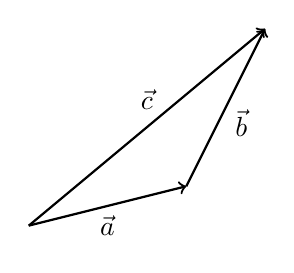
\begin{tikzpicture}        
        \draw[thick,->] (0,0) -- (2,0.5);
        \node at (1,0) {$\vec{a}$};
        \draw[thick,->] (2,0.5) -- (3,2.5);
        \node at (2.7,1.3) {$\vec{b}$};
        \draw[thick,->] (0,0) -- (3,2.5);
        \node at (1.5,1.6) {$\vec{c}$};
    \end{tikzpicture}
    \caption{Adding arrows.} \label{fig:vector-addition}
\end{figure}

Scaling a vector (multiplying it by a number) just alters its length without changing its direction, e.g. multiply by $0.5$ to shrink the vector to half its prior length.

We also learn about the dot product, a scalar-valued operator between two vectors, $\vec{p}\cdot\vec{q}$. If the two vectors $\vec{p}$ and $\vec{q}$ are separated by angle $\theta$, and we know the magnitude (length) of each vector, e.g. $\|\vec{p}\|$, then:

$$
\vec{p}\cdot\vec{q} = \|\vec{p}\| \|\vec{q}\|\cos{\theta}
$$

When we get onto the abstract definition of a vector it may seem like the geometric viewpoint has been relegated to a special case, less fundamental. But it is often useful to keep it in your mind as a way to visualise vectors of any kind, because however abstractly they are defined, they will always be closely analogous to the familiar arrows.

\subsection{Columns of numbers}

The second concrete way to think of vectors is as columns of ordinary numbers, and the number of \textit{dimensions} of the space tells us how many numbers a column vector has to contain. In this form, to add two vectors we just deal with the rows separately: add the numbers in row $1$, and then the numbers in row $2$ and so on for however many rows there are in a column vector, and thus obtain the sum as a column:

$$
\begin{bmatrix}2 \\ 0.5\end{bmatrix} +
\begin{bmatrix}1 \\ 2\end{bmatrix} =
\begin{bmatrix}3 \\ 2.5\end{bmatrix}
$$

More succinctly we can use index notation $a_n$ to mean the value in the $n$th row of the column associated with vector $\vec{a}$, so to add two vectors we just do this:

$$
a_n + b_n = c_n
$$

Scaling a vector just involves multiplying all the rows by the same number:

$$
d_n = x a_n
$$

The dot product is extremely simple in this representation: like with addition, you treat each row separately, multiplying the numbers in row $1$ and so on, but then you just sum all the products to get the numeric value:

$$
\sum_n a_n b_n
$$

\subsection{Coordinates}

These two perspectives are united by introducing a coordinate grid (Figure \ref{fig:vector-coordinate-grid}).

\begin{figure}[h]
    \centering
    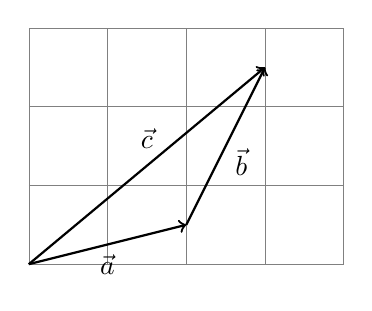
\begin{tikzpicture}       
        \draw[step=1cm,gray,very thin] (0,0) grid (4,3); 
        \draw[thick,->] (0,0) -- (2,0.5);
        \node at (1,0) {$\vec{a}$};
        \draw[thick,->] (2,0.5) -- (3,2.5);
        \node at (2.7,1.3) {$\vec{b}$};
        \draw[thick,->] (0,0) -- (3,2.5);
        \node at (1.5,1.6) {$\vec{c}$};
    \end{tikzpicture}
    \caption{Coordinate grid.} \label{fig:vector-coordinate-grid}
\end{figure}

Much of this subject is concerned with ensuring that our choice of coordinate grid doesn't get confused with the physical facts. We're trying to get answers about nature, and those answers better not change just because we used a different coordinate grid. One of the most important ideas in physics is that vectors are primarily geometric objects. They can be described with numeric coordinates, but there is no preferred coordinate basis. A vector has an independent existence, because it describes something in the physical world.

But however abstract things get, it can often be helpful to remember that you can visualise vectors as arrows and think of the basic operations on them geometrically, and equally it can be helpful to remember that we will always have a way of representing vectors as columns of numbers (indeed, columns of numbers \textit{are} vectors.)

The primary intuition we've been implicitly relying on so far is \textit{orthonormality}. With arrow vectors we can simply see when they are orthogonal, or to be more precise we can measure the angle between vectors, and we can measure their lengths, and we can choose a unit length, and so on. We can simply draw a unit vector, and then draw another unit vector that is orthogonal to it.

Likewise from the column vectors we have no difficult choosing a set of orthonormal vectors. They have a single row that contains $1$ and the other rows all contain $0$. In an $n$-dimensional space there can only be $n$ such distinct vectors.

None of these intuitive leaps will be available with abstract vector spaces, and orthonormality cannot be used as an elemental building block. Instead we will have to build towards it from more fundamental concepts.

By the way, when in physics we speak of a \textit{vector field}, that is, a vector at each point in space, such as wind speed and direction, or the electric field, we visualise arrows spread out over space. But the value of the field in two different places may be the same.

This is obvious (and less confusing) in the case of a scalar field, such as temperature. At two different locations in a room, the temperature may be the same. It's a numerical value that varies from place to place, and the same number may appear in two places.

But exactly the same is true for a vector field. If the wind is some particular speed and direction at two different places on the map, we say the vectors are equal: they are the \textit{same vector}. From the point of view of considering their equality, it is irrelevant that they are associated with different locations in physical space. In vector space, there is one vector with that direction and length.

On to the abstract stuff.

\section{Vectors as elements of a vector space}\label{sec:vectors-space}

A vector space is a set of objects, called vectors, about which we assume nothing except that we can perform certain operations on them.

\subsection{They can be added}

There is an operator $+$ that takes two objects from the set and returns another from the same set (we say it's a \textit{closed} operator).

This operator is commutative:

$$\vec{u} + \vec{v} = \vec{v} + \vec{u}$$

and associative:

$$\vec{u} + (\vec{v} + \vec{w}) = (\vec{v} + \vec{u}) + \vec{w}$$

There is a special object called $0$ (the \textit{zero vector}), which makes no difference when added to any object from the set:

$$\vec{v} + 0 = \vec{v}$$

Also every object has an opposite, known as its additive inverse, so they pair up. The inverse of $\vec{v}$ is written as $-\vec{v}$, and:

$$\vec{v} + (-\vec{v}) = 0$$

The above can written as $\vec{v} - \vec{v}$. Evidently $0$ is its own inverse.

Referring back to schoolhouse vectors, we can see how the arrows and the columns have an addition operation that satisfies all these requirements.

\subsection{They can be scaled}

There is an associated set of objects called scalars, typically restricted to real or complex numbers. Our objects can be multiplied by a scalar to get another object. Scaling them by $1$ makes no difference. Scaling them by $-1$ discovers the additive inverse.

Given two scalars $a$ and $b$, we can compute $c = ab$ and then scale an object $\vec{v}$ by it, or we can separately scale the object first by $a$ and then by $b$, and the result is the same:

$$(ab)\vec{v} = a(b\vec{v})$$

Scaling is distributive over addition of objects:

$$a(\vec{u} + \vec{v}) = a\vec{u} + a\vec{v}$$

And also over addition of scalars:

$$(a + b)\vec{v} = a\vec{v} + b\vec{v}$$

Again, arrows and columns have no problem meeting these requirements.

\subsection{Other Examples of Vector Spaces}

Any set of objects for which we can define these operations is a vector space, not just arrows and columns. The set of ordered tuples of real numbers $\mathbb{R}^n$ is just the column vectors with $n$ rows each. Also there is no reason why $n$ shouldn't be $1$, which means that the plain old set of real numbers $\mathbb{R}$ is also vector space. Think of the real number line as My First Vector Space\texttrademark.

Also the complex numbers $\mathbb{C}$, and tuples of them $\mathbb{C}^n$, work just as well. The example of $\mathbb{C}$ as a vector space is particularly interesting because of its close similarly to $\mathbb{R}^2$. The major difference is that it has a definition of multiplication as a closed operation over its vectors (such that the product of two vectors is a vector), which is absolutely not a general feature of vector spaces.\footnote{Although it is also defined (very differently) in $\mathbb{R}^3$ as the cross product, $\times$.}

In quantum mechanics we will contend with infinite-dimensional complex vector spaces.

\subsection{Fields}

The kind of set that can serve as a scalar is called a \textit{field}, which is a set of objects on which we have defined addition, subtraction, multiplication and division, so real or complex numbers usually serve this purpose (and always do in physics), but vectors in general cannot serve as a field of scalars for other vector spaces, because the definition of a vector space says nothing about there being a natural way to multiply or divide pairs of vectors to obtain other vectors.

In the same way, you can't have a vector space of $\mathbb{R}$ over the field of $\mathbb{C}$, because although we can use regular multiplication to "scale" a vector from $\mathbb{R}$ by a scalar from $\mathbb{C}$, the result is likely to be a member of $\mathbb{C}$ but not of $\mathbb{R}$, and thus not a vector from the same space.

Unless we say otherwise, we'll assume the field is $\mathbb{R}$.

\subsection{Finding a Basis}

If we select two vectors $\vec{a}$ and $\vec{b}$ from the space, we may find that they only differ by a scalar ratio $x$:

$$
\vec{b} = x \vec{a}
$$

If there is an $x$ that can scale $\vec{a}$ into $\vec{b}$ then those two vector are \textit{colinear}\footnote{This literally means "on the same line". Note the interesting use of geometrical language, even though we're not supposed to be thinking about arrows in this abstract discussion} (we are careful not to say they point in the same direction because if $x$ is negative then they point in exactly opposite directions, but are still colinear.)

But if there is no such $x$ then they are not colinear. This gives them an interesting superpower:

$$
\vec{r} = x \vec{a} + y \vec{b}
$$

By varying the scalar coefficients $x$ and $y$ we can construct any vector $r$ in a two-dimensional \textit{subspace} of the vector space.

Then suppose we look for a third vector $z$ that is not colinear with $x$ or $y$. Now we can construct any vector in three dimensions:

$$
\vec{r} = x \vec{a} + y \vec{b} + z \vec{c}
$$

Eventually we may find (assuming the space is finite dimensional) that it is not possible to find another vector that is not colinear with all of the $\vec{a}, \vec{b}, \vec{c}, ...$ we've discovered. The number of vectors in this set of mutually non-colinear vectors tells us how many dimensions the space has, and these vectors are said to \textit{span} the space.

The vitally important thing to realise about this is that at no point have we said that these vectors are orthogonal. We haven't even defined what that means yet. We've only defined the property of being colinear. Nevertheless we have arrived at the idea of a coordinate grid; it's just that our grid may be awkwardly slanted, made of identical parallelogram tiles rather than identical square tiles.

So we don't have to keep choosing letters, we will label each dimension with a number. The set of mutually non-colinear vectors that we can use to construct any other vector in the space is called a \textit{basis}. The basis vectors are traditionally written as $\vec{e}_n$, where $n$ is often 1-based (although in relativity it is usually 0-based). The scalar coefficients that construct a given vector $r$ can also be numbered, conventionally with superscript $r^n$:

\begin{equation}
\begin{split}
\vec{r} &= r^1 \vec{e}_1 + r^2 \vec{e}_2 + ... + r^n \vec{e}_n \\
        &= \sum_n r^n \vec{e}_n
\end{split}
\end{equation}

The use of a superscript index is obviously asking for trouble given that it looks like we're raising $r$ to a power, but this notation is universal in physics so we may as well get used to it.

Having chosen a basis, we can describe any vector with a tuple of scalar coefficients $r_n$, so any vector space of dimension $N$ whose scalar field is $\mathbb{F}$ must be isomorphic with $\mathbb{F}^N$. In other words, all vectors can be described by column vectors, but the numbers in the columns will depend on our choice of basis.

But the laws of physics cannot possibly care what basis we choose, so we need ways of obtaining numeric facts about vectors that do not depend on the choice of basis.

\section{Covectors}

Think of a scalar-valued function of a vector. That is, a black box with a single input slot accepting a vector $\vec{a}$, and an output hole that gives us back a scalar $x$ (Figure \ref{fig:1-slot-box}).

\begin{figure}[h]
    \centering
    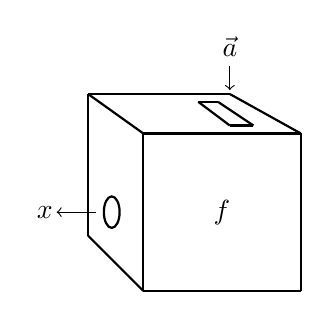
\begin{tikzpicture}
        \draw[thick] (0,0) -- (2,0);
        \draw[thick] (2,0) -- (2,2);
        \draw[thick] (2,2) -- (0,2);
        \draw[thick] (0,2) -- (0,0);
        \draw[thick] (0,2) -- (-0.7,2.5);
        \draw[thick] (-0.7,2.5) -- (-0.7,0.7);
        \draw[thick] (-0.7,0.7) -- (0,0);
        \draw[thick] (-0.7,2.5) -- (1.1,2.5);
        \draw[thick] (1.1,2.5) -- (2,2);

        \draw[thick] (1.4,2.1) -- (0.95,2.4);
        \draw[thick] (0.95,2.4) -- (0.7,2.4);
        \draw[thick] (0.7,2.4) -- (1.1,2.1);
        \draw[thick] (1.1,2.1) -- (1.4,2.1);
        
        \node at (1.1,3.1) { $\vec{a}$};
        \draw[->] (1.1,2.85) -- (1.1,2.55);

        \node at (-1.25,1) { $x$};
        \draw[thick] (-0.4,1) ellipse (0.1 and 0.2);
        \draw[->] (-0.6,1) -- (-1.1,1);

        \node at (1,1) { $f$};

    \end{tikzpicture}
    \caption{Function $f$ with a single slot accepting a vector} \label{fig:1-slot-box}
\end{figure}

More precisely, this machine is a mapping from the vector space to the real numbers. There are infinitely many such mappings and they could be rather complicated. We will restrict ourselves to a simple subset of these mappings.

First, we note that it is possible to define the addition operator on mappings:

$$
f(\vec{a}) = g(\vec{a}) + h(\vec{a})
$$

That is, it could be that inside the box $f$, there are concealed two boxes $g$ and $h$. When $f$ receives an input vector $\vec{a}$, it passes it to both $g$ and $h$, and adds their results together to obtain its own result. Note that we haven't yet restricted the complexity of $g$ and $h$; we have no idea what they do to produce their individual results.

Likewise, it is possible to scale a mapping by a coefficient $x$:

$$
f(\vec{a}) = x g(\vec{a})
$$

The trick to restricting the complexity of our set of possible mappings is to require that they comply with the rules of a vector space. Not only can they be added and scaled, but combinations of these operations produce consistent results. But if we do that, then we have also ensured that the set of mappings actually \textit{is} a vector space, and furthermore, that each mapping must be a vector chosen from that space.

Note that we haven't proven that every possible mapping is a vector. We've merely restricted ourselves to only considering a subset of mappings, those that can be scaled and added to find other mappings from the same restricted subset, such that scaling a mapping by 5 is the same as scaling that mapping by 2 and separately by 3 and then adding those two scaled mappings.

If we label the original vector space $V$ then this associated vector space of mappings $V \mapsto \mathbb{R}$ is written as $V^*$ and is called the dual space of $V$. All we've discovered so far about $V$ also applies to $V^*$, including the idea of two mappings being non-colinear, which means we can select a basis made up of mutually non-colinear covectors chosen from $V^*$ and thus construct any mapping from it by scaling and adding the basis mappings. That's quite a leap, so pause to digest it. The moment you discover a set of objects is a vector space, you know you can choose a basis, and then describe anything in that space in terms of a weighted sum of that basis.

We call the mappings taken from $V^*$ \textit{covectors}. The basis covectors are labelled with superscripts $\vec{e}^n$ and the coefficients with subscripts $f_n$, so we can build any covector from the chosen basis:

\begin{equation}
    \begin{split}
    \vec{f} &= f_1 \vec{e}^1 + f_2 \vec{e}^2 + ... + f_n \vec{e}^n \\
            &= \sum_n f_n \vec{e}^n
    \end{split}
\end{equation}

It follows that, just as $N$-dimensional vectors are isomorphic with columns of $N$ scalars, so too are their associated covectors.

It is sometimes suggested that all vector spaces have a dual space, as if this was some property hiding in the definition of a vector space. But in truth we have conjured the dual space into existence, first by inventing the idea of a mapping $V \mapsto \mathbb{R}$, then by defining operations on those mappings, then by considering the set of all possible mappings, and finally by imposing the rules of vector spaces, which restricts us to a subset of the possible mappings that we named covectors. There is nothing particularly automatic about this. We made it happen by being curious about ways in which vectors might be paired with numbers.

Another important point to note is that as covectors are vectors, the operation we've been writing as $f(\vec{a})$ is in fact much more symmetrical than that notation implies. We take a vector $V$ and a covector from $V^*$ and this produces a scalar from $\mathbb{R}$. 

So we could equally say that a vector "operates" on a covector to produce the scalar. From the point of view of $V^*$ it is $V$ that is the dual space. There is a more symmetrical notation we can use to make this clear:

$$\langle \vec{f},\vec{a}\rangle$$

In this notation, the left and right sides of the operation are from mutually dual spaces.

\section{Connecting the Dual Spaces}

We obviously have a lot of freedom when choosing a basis in either $V$ or $V^*$. What can we usefully do to relate the two sides? We've seen how a covector is built as a weighted sum of basis vectors $\vec{e}^i$ from $V^*$:

$$
\vec{f} = \sum_i f_i \vec{e}^i
$$

Now consider how a randomly chosen $V^*$ covector $\vec{f}$ acts on a $V$ basis vector $\vec{e}_j$ to produce a scalar value. We'd like to arrange matters so that, whatever $\vec{f}$ is chosen, that scalar is the $f_j$ coefficient of the covector, so we can give the simple instruction: to obtain the $j$th component of any covector, let it act on the $j$th basis vector:

$$
f_j = \langle \vec{f} , \vec{e}_j\rangle
$$

If that's true then we can substitute $\vec{f}$ expressed as a sum:

$$
f_j = \langle \sum_i f_i \vec{e}^i , \vec{e}_j\rangle
$$

and linearity allows us to separately deal with each dimension and sum their results:

$$
f_j = \sum_i f_i \langle \vec{e}^i , \vec{e}_j\rangle
$$

But if that's true for \textit{any} $\vec{f}$, and not just a coincidence applying to some specific example, then the scalar factor $\langle \vec{e}^i , \vec{e}_j\rangle$ must be "selecting" just one of the $f_i$ terms, specifically the one where $i = j$, and eliminating all others, or to put it another way:

$$
f_j = \sum_i f_i \delta \indices{^i_j}
$$

So if the $f_j$ are indeed the components of the covector, discovered by making it act on the basis vectors, we've discovered the relationship that must exist between the dual bases:

\begin{equation}
    \langle \vec{e}^i,\vec{e}_j\rangle = \delta\indices{^i_j}
    \label{eqn:dual-bases-delta}
\end{equation}

So we could choose any basis at all in $V$, and then definition \eqref{eqn:dual-bases-delta} restricts the choice of basis in $V^*$, or vice versa. Such is the symmetry of this situation, we could instead have let a basis covector $\vec{e}^j$ act on a randomly chosen vector $\vec{a}$ and require that this give us the $j$th coordinate of $\vec{a}$, and we'd have reached the same conclusion.

From now on we'll assume that this alignment of the dual bases has been performed. That being the case, we can compute the action of a covector on a vector by arithmetic on their coefficients:

\begin{equation}
    \begin{split}
        \langle \vec{f},\vec{a}\rangle 
        &= \langle \sum_i f_i \vec{e}^i , \sum_j a^j \vec{e}_j \rangle \\
        &= \sum_{ij} f_i a^j \langle\vec{e}^i,\vec{e}_j\rangle \\
        &= \sum_{i} f_i a^i
    \end{split}
\end{equation}

So the linearity allows us to sum over all combinations of $i, j$ and pull the coefficients outside of the action of the covector on the vector, and the dual bases yield the value $1$ where $i = j$ and $0$ otherwise, so we just end up with a simple sum over the products of the paired-up coefficients.

In a roundabout way we've discovered the dot product, albeit between a covector and a vector rather than two ordinary vectors. We still haven't introduced any concept of orthonormality, or even orthogonality, between pairs of vectors. Our "coordinate grid" is still not necessarily a lattice of squares, and our dot product is between elements of two different vector spaces, but we always choose their basis vectors so they are related by a definite requirement, which we can state in two ways:

\begin{enumerate}
    \item The $n$th basis covector from $V^*$ can be used to extract the $n$th coefficient of a vector from $V$.
    \item The $n$th basis vector from $V$ can be used to extract the $n$th coefficient of a covector from $V^*$.
\end{enumerate}

And as a consequence of this (dual) requirement we find that when the $n$th basis covector acts on the $m$th basis vector, the result is $1$ if $m = n$ and $0$ if $m \ne n$.

If we describe our covectors and vectors as sets of coefficients, to make a covector act on a vector we simply perform the dot product between their coefficients. Or equivalently, we write the covector as a single row matrix on the left, and the vector as a single column matrix on the right, and perform matrix multiplication to get a single scalar.

It may be worth pausing here to see how this result relates to our schoolhouse version of arrows and coordinates and the dot product. In that world-view, the coordinates are just the coefficients that multiply by the orthonormal basis vectors to construct a vector, and the dot product of a basis vector $\vec{e}_i$ and a given vector $\vec{a}$ produces the $a_i$ coordinate of $\vec{a}$. This is how we understand the geometric dot product (with $\cos \theta$) to be related to the idea of simply plucking one of the numbers from a column vector.

But what happens if the unit basis vectors aren't orthogonal? If we have non-orthogonal basis vectors (Figure \ref{fig:vectors-non-orth-1}) we can still sum them to generate any vector in the space (Figure \ref{fig:vectors-non-orth-2}).

\begin{figure}[h]
    \caption{Building a vector from a non-orthogonal basis}
    \begin{subfigure}{0.5\textwidth}
        \centering
        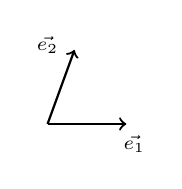
\begin{tikzpicture}
            \node at (1.1,-0.25) {\scriptsize $\vec{e_1}$};
            \draw[thick,->] (0,0) -- (0.342,0.940);
            \node at (0,1) {\scriptsize $\vec{e_2}$};
            \draw[thick,->] (0,0) -- (1,0);
        \end{tikzpicture}
    \caption{Non-orthogonal basis $\vec{e}_n$} \label{fig:vectors-non-orth-1}
    \end{subfigure}
    \begin{subfigure}{0.5\textwidth}
        \centering
        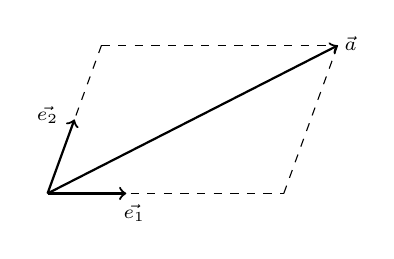
\begin{tikzpicture}
            \draw[dashed] (0,0) -- (3,0);
            \draw[dashed] (3,0) -- (3.684,1.879);
            \draw[dashed] (0,0) -- (0.684,1.879);
            \draw[dashed] (0.684,1.879) -- (3.684,1.879);
            \node at (1.1,-0.25) {\scriptsize $\vec{e_1}$};
            \draw[thick,->] (0,0) -- (0.342,0.940);
            \node at (0,1) {\scriptsize $\vec{e_2}$};
            \draw[thick,->] (0,0) -- (1,0);                    
            \draw[thick,->] (0,0) -- (3.684,1.879);
            \node at (3.85,1.9) {\scriptsize $\vec{a}$};
        \end{tikzpicture}
        \caption{$\vec{a} = \vec{e}_1 a^1 + \vec{e}_2 a^2$} \label{fig:vectors-non-orth-2}
    \end{subfigure}
\end{figure}

The problem comes when we try to recover the coordinates by projecting $\vec{a}$ onto the two basis vectors (Figure \ref{fig:vectors-non-orth-3}).

\begin{figure}[h]
    \caption{Projecting a vector onto a non-orthogonal basis}
    \begin{subfigure}{0.5\textwidth}
        \centering
        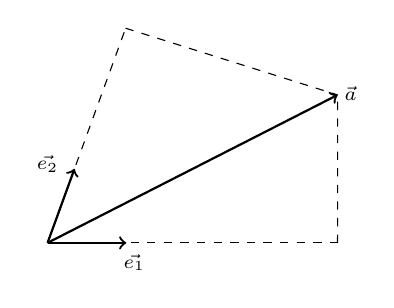
\begin{tikzpicture}
            \draw[dashed] (0,0) -- (3.684,0);
            \draw[dashed] (3.683,0) -- (3.684,1.879);
            \draw[dashed] (0,0) -- (0.992,2.726);
            \draw[dashed] (0.992,2.726) -- (3.684,1.879);
            \node at (1.1,-0.25) {\scriptsize $\vec{e_1}$};
            \draw[thick,->] (0,0) -- (0.342,0.940);
            \node at (0,1) {\scriptsize $\vec{e_2}$};
            \draw[thick,->] (0,0) -- (1,0);                    
            \draw[thick,->] (0,0) -- (3.684,1.879);
            \node at (3.85,1.9) {\scriptsize $\vec{a}$};
        \end{tikzpicture}
    \caption{Projecting $\vec{a}$ back onto the basis} \label{fig:vectors-non-orth-3}
    \end{subfigure}
    \begin{subfigure}{0.5\textwidth}
        \centering
        \begin{tikzpicture}
            \draw[dashed] (0,0) -- (3.684,-1.339);
            \draw[dashed] (3.683,-1.339) -- (3.684,1.879);
            \draw[dashed] (0,0) -- (0,3.218);
            \draw[dashed] (0,3.218) -- (3.684,1.879);
            \node at (1.2,-0.20) {\scriptsize $\vec{e^1}$};
            \draw[thick,->] (0,0) -- (0,1);
            \node at (-0.2,1.2) {\scriptsize $\vec{e^2}$};
            \draw[thick,->] (0,0) -- (0.992,-0.342);                    
            \draw[thick,->] (0,0) -- (3.684,1.879);
            \node at (3.85,1.9) {\scriptsize $\vec{a}$};
        \end{tikzpicture}
        \caption{$\vec{a} = a_1 \vec{e^1} + a_2 \vec{e^2}$} \label{fig:vectors-non-orth-4}
    \end{subfigure}
\end{figure}

We can visualise this projection process by drawing lines from the tip of $\vec{a}$ so they meet at right angles with the lines extended from the basis vectors. But these imply different coordinates for $\vec{a}$ from the ones that we used to build it using the basis $\vec{e}_n$.

This raises the question: in what basis are these the coordinates for $\vec{a}$? There is such a basis (Figure \ref{fig:vectors-non-orth-4}), $\vec{e^n}$, and we label the coordinates with subscripts, $a_n$, so the reconstructed $\vec{v}$ is given by:

$$
\vec{a} = a_1 \vec{e^1} + a_2 \vec{e^2}
$$

This basis $\vec{e}_j$ is related to the original basis $\vec{e}^i$ by \eqref{eqn:dual-bases-delta}. In other words, when choosing the dual basis vector for a given index, we must choose a vector that is orthogonal to all the other basis vectors, and this means we will have a severely limited choice, because there can be only one alignment that meets this requirement. Furthermore the magnitude of the vector $\vec{e}^i$ is fully determined by the requirement that $\vec{e}_i \cdot \vec{e}^i = 1$, as the ratio between the coordinates is already fixed by the choice of alignment.

In this visualisation process we have shown the relationship between $V$ and $V*$ by overlaying them on the same diagram, but they are in fact separate vector spaces: elements of $V$ are not elements of $V*$, and vice versa. But the way we have calibrated these two sets of bases to be mutually consistent is exactly the same as the relationship between the bases of $V$ and $V*$.

If the original basis vectors had been orthogonal, the dot product would have produced exactly the same coordinates we'd used to build the vector in the first place, i.e. figures \ref{fig:vectors-non-orth-2}, \ref{fig:vectors-non-orth-3} and \ref{fig:vectors-non-orth-4} would all be identical: a rectangle with the vector as its diagonal.

\section{More slots}

Let's upgrade our black box machine so it has two input slots, accepting vectors $\vec{a}$ and $\vec{b}$ from the same vector space $V$, but still one output hole that gives us back a scalar $x$ (Figure \ref{fig:2-slot-box}).

\begin{figure}[h]
    \centering
    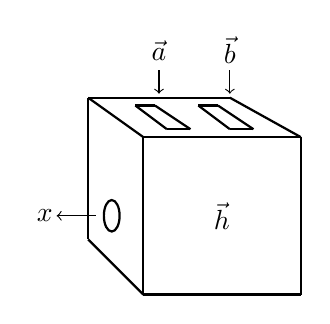
\begin{tikzpicture}
        \draw[thick] (0,0) -- (2,0);
        \draw[thick] (2,0) -- (2,2);
        \draw[thick] (2,2) -- (0,2);
        \draw[thick] (0,2) -- (0,0);
        \draw[thick] (0,2) -- (-0.7,2.5);
        \draw[thick] (-0.7,2.5) -- (-0.7,0.7);
        \draw[thick] (-0.7,0.7) -- (0,0);
        \draw[thick] (-0.7,2.5) -- (1.1,2.5);
        \draw[thick] (1.1,2.5) -- (2,2);

        \draw[thick] (1.4,2.1) -- (0.95,2.4);
        \draw[thick] (0.95,2.4) -- (0.7,2.4);
        \draw[thick] (0.7,2.4) -- (1.1,2.1);
        \draw[thick] (1.1,2.1) -- (1.4,2.1);

        \draw[thick] (0.6,2.1) -- (0.15,2.4);
        \draw[thick] (0.15,2.4) -- (-0.1,2.4);
        \draw[thick] (-0.1,2.4) -- (0.3,2.1);
        \draw[thick] (0.3,2.1) -- (0.6,2.1);
        
        \node at (0.2,3.1) { $\vec{a}$};
        \draw[->] (0.2,2.85) -- (0.2,2.55);

        \node at (1.1,3.1) { $\vec{b}$};
        \draw[->] (1.1,2.85) -- (1.1,2.55);

        \node at (-1.25,1) { $x$};
        \draw[thick] (-0.4,1) ellipse (0.1 and 0.2);
        \draw[->] (-0.6,1) -- (-1.1,1);

        \node at (1,1) { $\vec{h}$};

    \end{tikzpicture}
    \caption{Box $\vec{h}$ with two slots accepting vectors} \label{fig:2-slot-box}
\end{figure}

This is a mapping from pairs of vectors to $\mathbb{R}$. In another act of spectacular laziness we we restrict ourselves to considering mappings that can be implemented as follows.

Inside the box $\vec{h}$, there are two single-slot boxes (covectors) $\vec{f}$ and $\vec{g}$. The machinery inserts $\vec{a}$ into box $\vec{f}$, and $\vec{b}$ into box $\vec{g}$, to obtain two scalars, which it simply multiplies together to produce its own resultant scalar that falls out of the hole of $\vec{h}$. In other words, it's really just two covectors glued together by scalar multiplication.

This mechanism is \textit{bilinear}, meaning that if either one of $\vec{f}$ or $\vec{g}$ were to be scaled by some factor $y$, the output of $\vec{h}$ would also be scaled by $y$.

The notation for constructing this machine from two covectors is $V^* \otimes V^*$. On seeing that notation, think of each $V^*$ as a slot $\vec{f}$ that is waiting for a vector $\vec{a}$ from $V$ to arrive, so it can make the scalar value $\langle \vec{f},\vec{a}\rangle$. Both slots will do that, and then the resulting scalars are multiplied.

Suppose we've chosen the covectors $\vec{f}$ and $\vec{g}$, so the machinery is:

$$
\vec{h}(\vec{a}, \vec{b}) = \langle \vec{f},\vec{a}\rangle \langle \vec{g},\vec{b}\rangle
$$

We know that covectors can be expressed as a weighted sum of a basis:

$$
\vec{f} = \sum_i f_i \vec{e}^i
$$

And likewise for vectors:

$$
\vec{a} = \sum_i a^i \vec{e}_i
$$

So we can substitute to get this mess:

$$
\vec{h}(\vec{a}, \vec{b}) = 
\langle\sum_i f_i \vec{e}^i,\sum_j a^j \vec{e}_j\rangle 
\langle\sum_k g_k \vec{e}^k,\sum_l b^l \vec{e}_l\rangle
$$

But linearity means we can write:

$$
\vec{h}(\vec{a}, \vec{b}) = 
\left(\sum_{ij} f_i a^j \langle\vec{e}^i,\vec{e}_j\rangle \right)
\left(\sum_{kl} g_k b^l \langle\vec{e}^k,\vec{e}_l\rangle \right)
$$

And \eqref{eqn:dual-bases-delta} implies:

$$
\vec{h}(\vec{a}, \vec{b}) = \left(\sum_{i} f_i a^i \right) \left(\sum_{k} g_k b^k \right)
$$

Multiplying out, we get:

$$
\vec{h}(\vec{a}, \vec{b}) = \sum_{ik} f_i g_k a^i b^k
$$

It seems the fixed coefficients of $\vec{f}$ and $\vec{g}$ can be collapsed into a single matrix $M$ whose elements $M_{ik}$ give us the weighting to apply to each possible product of vector coefficients $a^i b^k$.

$$
M_{ik} = f_i g_k
$$

So to represent a two-slot machine with respect to a chosen basis (and corresponding dual basis), we need a matrix.

Another way to approach this is to consider the space of all possible pairs of covectors $V^* \times V^*$. We can define addition and scaling on these pairs in a way that satisfies the requirements of a vector space, and thus we have defined a vector space. We can form a basis for that space by taking all possible pairs of basis covectors, $\vec{e}^i \times \vec{e}^j$. If the space is $N$-dimensional, the pair-space will be $N^2$-dimensional. This is the space of all possible two-slot machines. And therefore to describe any two-slot machine in terms of that basis we will need $N^2$ coefficients, which we can arrange into a square of $N$ rows and $N$ columns.

\section{The Inner Product}

The most important use case of a specific machine of the form $V^* \otimes V^*$ is to serve the same purpose as the simple dot product, except without the requirement that the basis must be an orthonormal basis, because in our abstract vector spaces, we still haven't said what that means.

Nominating one such machine for a given vector space, we can call it the \textit{inner product}, and we say that the combination of the vector space and its inner product is an \textit{inner product space}.

The notation $(\vec{a},\vec{b})$ is sometimes used for the inner product, similar to but deliberately distinct from the $\langle \vec{f},\vec{a}\rangle$ notation for the action of a covector on a vector.\footnote{Sadly the meanings of these notations are sometimes switched, and they aren't the only notations used.}

As we've seen, as its a two-slot machine, its coordinate representation will be a matrix. In General Relativity this matrix is usually called $g$, and its indices are $\mu$ and $\nu$, so applying it to vectors $\vec{a}$ and $\vec{b}$ will look like this:

$$
(\vec{a},\vec{b}) = \sum_{\mu\nu} g_{\mu\nu} a^\mu b^\nu
$$

It's worth pausing to compare it to the familiar dot product, which would be:

$$
\vec{a} \cdot \vec{b} = \sum_{\mu} a^\mu b^\mu
$$

Only one index summed over instead of two, and no scaling of the contribution from the summed terms. So the dot product is like the general inner product but with $g$ replaced with the Kronecker delta (§\ref{def:Kronecker}):

$$
g_{\mu\nu} = \delta_{\mu\nu}
$$

So in comparison with the dot product, the general form of the inner product, or specifically the matrix $g_{\mu\nu}$, captures something about the non-orthonormality of the basis. If it were perfectly orthonormal then $g_{\mu\nu}$ would be the identity matrix and we'd be able to use the dot product as our inner product.

This is exactly what we saw with the dual parallelograms resulting from trying to project onto a non-orthogonal basis.

We can make this concrete by playing with $\mathbb{R}^2$ as our vector space $V$, in which case the dual space of covectors $V^*$ is $\mathbb{R}^2 \mapsto \mathbb{R}$.

\begin{figure}[h]
    \caption{Basis vectors in $\mathbb{R}^2$}
    \begin{subfigure}{0.5\textwidth}
        \centering
        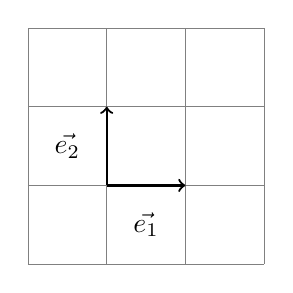
\begin{tikzpicture}
            \draw[step=1cm,gray,very thin] (1,1) grid (4,4); 
            \draw[thick,->] (2,2) -- (3,2);
            \node at (2.5,1.5) {$\vec{e_1}$};
            \draw[thick,->] (2,2) -- (2,3);
            \node at (1.5,2.5) {$\vec{e_2}$};        
        \end{tikzpicture}
        \caption{Orthonormality} \label{fig:vectors-orthonormality}
    \end{subfigure}
    \begin{subfigure}{0.5\textwidth}
        \centering
        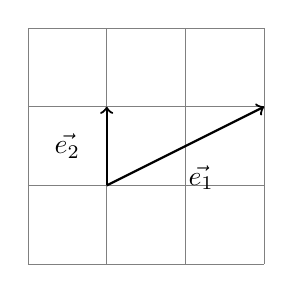
\begin{tikzpicture}
            \draw[step=1cm,gray,very thin] (1,1) grid (4,4); 
            \draw[thick,->] (2,2) -- (4,3);
            \node at (3.2,2.1) {$\vec{e_1}$};
            \draw[thick,->] (2,2) -- (2,3);
            \node at (1.5,2.5) {$\vec{e_2}$};
        \end{tikzpicture}
        \caption{Awkwardness} \label{fig:vectors-awkwardness}
    \end{subfigure}
\end{figure}

It would be easy to choose an orthonormal basis in $\mathbb{R}^2$ (Figure \ref{fig:vectors-orthonormality}):

$$
e_1 = \begin{bmatrix}1 \\ 0\end{bmatrix}\,,\,
e_2 = \begin{bmatrix}0 \\ 1\end{bmatrix}
$$

But we'll be awkward and act like we don't know what orthonormal means (Figure \ref{fig:vectors-awkwardness}):

$$
e_1 = \begin{bmatrix}2 \\ 1\end{bmatrix}\,,\,
e_2 = \begin{bmatrix}0 \\ 1\end{bmatrix}
$$

By the way, it is customary to put the basis vectors in a row matrix, $\begin{bmatrix}\vec{e}_1 & \vec{e}_2\end{bmatrix}$, so they can be matrix-multiplied by a column representation of a vector in $V$, but that's not what we're doing here. We are giving the definition of each basis vector in $V$ as a $1$-dimensional matrix, and the basis vectors are ordinary vectors belonging to $V$, so they must be column matrices.

What is the corresponding $V^*$ basis, $e^i$? It has to obey:

$$
\langle e_j,e^i \rangle = \delta \indices{_i^j}
$$

Some straightforward equation building and substitution yields:

$$
e^1 = \begin{bmatrix}0.5 & 0\end{bmatrix}\,,\,
e^2 = \begin{bmatrix}-0.5 & 1\end{bmatrix}
$$

And these being covectors from $V^*$, they must be row matrices, as shown. Using our $V$ basis we can construct the vector $\vec{v}$ from the coefficients $(2, 3)$:

$$
\vec{v} = 2e_1 + 3e_2
        = \begin{bmatrix}4 \\ 2\end{bmatrix} + \begin{bmatrix}0 \\ 3\end{bmatrix} 
        = \begin{bmatrix}4 \\ 5\end{bmatrix}
$$

What happens if we evaluate the $V^*$ basis functions against $\vec{v}$?

$$
\begin{bmatrix}0.5 & 0\end{bmatrix} \begin{bmatrix}4 \\ 5\end{bmatrix} = 2 
\,,\,
\begin{bmatrix}-0.5 & 1\end{bmatrix} \begin{bmatrix}4 \\ 5\end{bmatrix} = 3
$$

We get back the correct coefficients. If we'd just transposed the $V$ basis vectors into rows and left-multiplied them, we would have obtained wrong answers: this is precisely the same problem we saw with projecting onto the non-orthogonal basis.

So much for using the dual basis to get the right answers, but with the inner product we can forget the existence of the dual basis. Instead of having to think of our set of basis vectors $\vec{e}_n$ having corresponding dual covectors $\vec{e}^n$, we instead conceal this detail inside the machinery of a two-slot function that produces a scalar value from any two vectors, the same value we'd get if the basis was orthogonal and we used the regular dot product.

We know the machinery will consist of a matrix, which we can (for the moment, naively) think of as "fixing" a basis vector to be like its dual. What matrix $g_{\mu\nu}$ converts $\vec{e}_n$ into $\vec{e}^n$? Continuing our simple $2$-dimensional example, we'd have:

$$
g_{\mu\nu} \vec{e}_1 = \vec{e}^1 \,,\, g_{\mu\nu} \vec{e}_2 = \vec{e}^2
$$

or in matrix notation:

$$
\begin{bmatrix}g_{11} & g_{12} \\ g_{21} & g_{22}\end{bmatrix}
\begin{bmatrix}2 \\ 1\end{bmatrix} = 
\begin{bmatrix}0.5 \\ 0\end{bmatrix}
$$

and:

$$
\begin{bmatrix}g_{11} & g_{12} \\ g_{21} & g_{22}\end{bmatrix}
\begin{bmatrix}0 \\ 1\end{bmatrix} = 
\begin{bmatrix}-0.5 \\ 1\end{bmatrix}
$$

This is an easy simultaneous equation problem and the answer is:

$$
g_{\mu\nu} = \begin{bmatrix}0.5 & -0.5 \\ -0.5 & 1\end{bmatrix}
$$

So with our awkward basis, the correct form of the inner product, which we can use to extract (say) the first coordinate of $\vec{v}$ using the first basis vector $\vec{e}_1$, is:

$$
(\vec{v}, \vec{e}_1) =
\vec{v} g_{\mu\nu} \vec{e}_1 =
\begin{bmatrix}2 & 3\end{bmatrix} 
\begin{bmatrix}0.5 & -0.5 \\ -0.5 & 1\end{bmatrix}
\begin{bmatrix}2 \\ 1\end{bmatrix}
=
2
$$

But (to outgrow the naivety alluded to just now) the inner product has symmetry\footnote{Strictly speaking it has conjugate symmetry, but if scalars are real numbers then this is just symmetry.}: we can swap $\vec{v}$ and $\vec{e}_1$ without affecting the result. So there is no special treatment that specifically "fixes" the basis vector by producing its dual. (Indeed, neither of the arguments to the inner product needs to be a basis vector.) We could equally suppose that the matrix $g_{\mu\nu}$ "fixes" $\vec{v}$ to be a different vector so that the unmodified $\vec{e}_1$ can extract the expected value from it (and this is easily corroborated by the above example).

Having established an inner product, we can at last give a meaning to the length or \textit{norm} of a vector: it's the square root of the inner product of the vector with itself. Once again, if the basis is orthonormal then the mathematical machinery is immediately familiar: it's just the pythagoras theorem.

And we can finally say what we mean by an orthogonal pair of vectors, and an orthonormal basis. Two vectors are orthogonal if their inner product is zero. A basis is orthogonal if the basis vectors are mutually orthogonal. A basis is orthonormal if all the basis vectors are of norm $1$.

\section{Change of Basis}\label{sec:vectors-change-basis}

A matrix can be used to:

\begin{itemize}
    \item map vectors to a new length and direction in the same basis, or
    \item perform a coordinate conversion on vectors so they remain the same vectors but expressed in different numerical coordinates.
\end{itemize}

The mathematical machinery is identical.

Viewed as an operator, the matrix may have eigenvectors (lines along which vectors only change length, not direction) only in some directions. The operator is therefore a geometrical object just as a vector is, and the matrix elements may be numerically different depending on the basis, just as the coordinates of a vector may differ depending on the basis, despite describing the very same objects regardless of the basis chosen.

Viewed as a coordinate converter, the matrix effectively depends on two bases, the one being converted from and the one being converted to.

\subsection{Effect of change of basis on vectors}

A plane vector $\vec{v}$ in some basis can be expressed in coordinates as a column matrix $v$:

$$v = \begin{bmatrix}3 \\ 4\end{bmatrix}$$

Note that, unlike some prior examples, we are not saying the vector \textit{is} the column matrix. We are saying nothing at all about the nature of the vectors, except that they are elements of some vector space. We are describing in numbers a vector of unknown type taken from some vector space, which we can only do because we have chosen a basis, $e$:

$$e = \begin{bmatrix}\vec{e_1} & \vec{e_2}\end{bmatrix}$$

Matrix multiplication builds the vector:

$$\vec{v} = ev = 3\vec{e_1} + 4\vec{e_2}$$

We can create a matrix that will double the length of the basis vectors:

$$G = \begin{bmatrix}2 & 0 \\ 0 & 2\end{bmatrix}$$

By the rules of matrix multiplication the bases needs to be on the left:

$$e' = eG = \begin{bmatrix}2\vec{e_1} & 2\vec{e_2}\end{bmatrix}$$

What coordinates would $\vec{v}$ have in this new basis $e'$? Intuitively the coordinates need to be halved to refer to the same vector. So we need the inverse of $G$, written as $G^{-1}$, which shrinks the coordinates, so we'll call it:

$$S = G^{-1} = \begin{bmatrix}0.5 & 0 \\ 0 & 0.5\end{bmatrix}$$

And so our vector's coordinates become:

$$v' = Sv = \begin{bmatrix}1.5 \\ 2\end{bmatrix}$$

This is the same vector as before, just in different coordinates:

$$\vec{v} = ev = e'v'$$

We say that vectors are \textit{contravariant} under a change of basis.

\subsection{The inner product under change of basis}

We've gone to some trouble so far to define the inner product in such a way that it can produce consistent results even with awkward basis vectors. But the matrix $g_{\mu\nu}$ that defines it may need to be updated depending on the type of change we make to the basis.

If the vector space is rotated or reflected this preserves both lengths and angles, so the inner product between a given pair of vectors before and after that transformation will be the same. Operators that preserve the inner product are \textit{unitary}.

If the basis vectors are scaled, the lengths implied by the coordinates will change and so the inner product will change. To take the above example, we grow the basis vectors with $G$, having the equivalent effect on the coordinates to shrinking the input vectors with $S$ to half their original length, and so the unmodified (now incorrect) inner product would be be $\frac{1}{4}$ of its original value. It therefore needs to be updated to account for the new basis.

A covector can be thought of as a yardstick or a measuring device. By evaluating it with some vector parameter, you are taking a measurement of that vector. The simplest example would be if you wanted to measure the magnitude (length) of $\vec{x}$, in which case you'd use the covector containing an $\vec{f}$ that was a unit vector colinear (lying on the same line) with $\vec{x}$. By the definition of the dot product, the angle between the two vectors being $0$, and the length of $\vec{f}$ being defined as $1$, the resulting scalar would be the length of $\vec{x}$, just as we wanted.

So the ordinary vector $\vec{x}$ is represented by a column matrix $x$ of coordinates in our initial basis, and we left-multiply it by $S^{-1}$ to get it in a new coordinate system:

$$
x' = S^{-1} x
$$

For the covector $\vec{f}$, which is a row matrix $f$, we right-multiply by $S$:

$$
f' = f S
$$

This ensures that the two representations give us exactly the same numerical result when we evaluate the function on the vector, regardless of the basis:

$$
f(x) = f'(x')
$$

The answer to $\vec{f}(\vec{x})$ is a basis-independent physical fact. We can make this absolutely clear by working through the arithmetic with some awkward numbers. Let's suppose our vector $\vec{x}$ is initially represented by a column matrix $x$ of coordinates:

$$
x = \begin{bmatrix} 3 \\ 2 \end{bmatrix}
$$

Meanwhile the covector (function) $\vec{f}$ is represented by a row matrix $f$:

$$
f = \begin{bmatrix} 4 & 4 \end{bmatrix}
$$

To evaluate $\vec{f}$ on $\vec{x}$, we do matrix multiplication (between a row and a column \textit{in that order}, this is the dot product):

\begin{equation}
\begin{split}
    \vec{f}(\vec{x}) &= \begin{bmatrix} 4 & 4 \end{bmatrix} \begin{bmatrix} 3 \\ 2 \end{bmatrix} \\
    &= 12 + 8 \\
    &= 20
\end{split}
\end{equation}

Now let's distort our basis vectors in some peculiar way, with the transformation $S$:

$$
S = \begin{bmatrix}
    2 & 1 \\
    -4 & 3
\end{bmatrix}
$$

To get the coordinates of $\vec{x}$ in the new basis, we'll need the inverse matrix $S^{-1}$ (fortunately for a 2x2 matrix there's a simple rule for this):

$$
S^{-1} = \begin{bmatrix}
    0.3 & -0.1 \\
    0.4 & 0.2
\end{bmatrix}
$$

And so the coordinates $x'$ in the new basis are:

\begin{equation}
\begin{split}
x' &= \begin{bmatrix}
    0.3 & -0.1 \\
    0.4 & 0.2
\end{bmatrix} \begin{bmatrix}
    3 \\ 2
\end{bmatrix} \\
  &= \begin{bmatrix}
    0.9 - 0.2 \\ 1.2 + 0.4
\end{bmatrix} \\
  &= \begin{bmatrix}
    0.7 \\ 1.6
\end{bmatrix}
\end{split}
\end{equation}

We need to find $\vec{f}$ expressed in the corresponding dual basis, the row vector $f'$, such that $\vec{f}(\vec{x})$ is still $20$. We're still asking the same question of the same vector, so we must get the same answer. To ensure this, we transform the row vector $f$ by multiplying on the right by the matrix $S$, that is, the same matrix we used to distort the basis vectors (this suggests that the dual basis vectors must have been distorted by $S^{-1}$, which is indeed the case):

\begin{equation}
\begin{split}
f' &= \begin{bmatrix}
    4 & 4
\end{bmatrix} \begin{bmatrix}
    2 & 1 \\
    -4 & 3
\end{bmatrix} \\
  &= \begin{bmatrix}
    8 - 16 & 4 + 12
\end{bmatrix} \\
  &= \begin{bmatrix}
    -8 & 16
\end{bmatrix}
\end{split}
\end{equation}

And we can finally check what we get when we evaluate $f(\vec{x})$ in these new coordinate representations:

\begin{equation}
\begin{split}
    \vec{f}(\vec{x}) &= \begin{bmatrix} -8 & 16 \end{bmatrix} \begin{bmatrix} 0.7 \\ 1.6 \end{bmatrix} \\
    &= -5.6 + 25.6 \\
    &= 20
\end{split}
\end{equation}

So a covector is a measuring device, a yardstick, always defined by a row vector, always working via the dot product (that is, matrix multiplication with a column vector), and so as to balance the effect of a coordinate transformation so the measurement remains the same, whatever we do to the coordinates of our vectors, we must do the inverse to the coordinates of our covectors.

If the transformation is a simple scaling up, it is pretty trivial to see that each vector coordinate will grow by a factor, and thus each covector coordinate must shrink by the same factor so that we get the same product when corresponding coordinates are multiplied. But the example above demonstrates how the same is true for any transformation described by a matrix.

Harking back once again to schoolhouse vectors, there is one situation in which this entire conclusion can be ignored, and it is both convenient and a source of confusion. To follow the rules of matrix multiplication, we have to put the matrix on the right of a column and on the left of a row:

\begin{equation}
    \begin{split}
        x' &= S^{-1} x \\
        f' &= f S        
    \end{split}
\end{equation}

We can switch the order in either line, but only if we also transpose all the matrices, which in the covector case turns rows into columns:

$$
f'^T = S^T f^T 
$$

As a column vector is now being left-multiplied by a matrix, this much more closely resembles the transformation for the ordinary vector, except that instead of $S^{-1}$ it uses $S^T$. But suppose $S$ is a unitary transformation (rotation or reflection, with no scaling or shearing). In that case:

$$
S^T = S^{-1}
$$

And so the transformation rule becomes:

$$
f'^T = S^{-1} f^T 
$$

So it is in fact identical to the formula for an ordinary vector. Under a unitary change of basis, we can represent covectors by column vectors and they transform exactly the same as ordinary vectors. It is only necessary to treat them differently if we allow non-unitary coordinate changes.

If you begin with an orthonormal basis, and apply a unitary transformation to your vector space, the basis will remain orthonormal. Hence another common name for a unitary transformation: an orthonormal transformation.

\section{Displacement in a scalar field}

We often have a scalar field (in the physics sense), that is, a scalar-valued function of position in space. An example is a survey of the temperature at points on a tabletop. This is highly unlikely to be a linear function of position. At one spot on the table there is a hot cup of tea, and on another there is an ice bucket of champagne. The temperature is a complex, messy function of position.

We can then ask what by what amount does the temperature change if we move from our current position to another spot nearby. This temperature change is given by a scalar-valued function of the displacement vector. Clearly this function has a different definition at each location. Also to be accurate over any distance it would need to be arbitrarily complicated.

The position of a point on the tabletop is given by a position vector and the temperature by the function $f$. We start at the point $\mathcal{P}$, reached by the position vector $\vec{p}$, where the temperature is $f(\vec{p})$, and we want to know by how much the temperature will change if we move by a small displacement $\vec{x}$.

\begin{figure}[h]
    \centering
    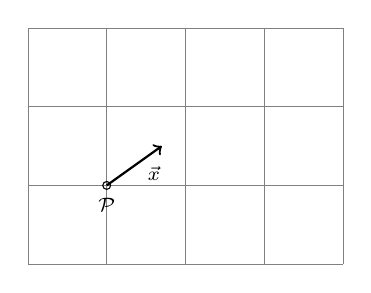
\begin{tikzpicture}
        \draw[step=1cm,gray,very thin] (0,0) grid (4,3);
        \node at (1,0.75) {\scriptsize $\mathcal{P}$};
        \draw (1,1) circle (0.05);
        \node at (1.6,1.15) {\scriptsize $\vec{x}$};
        \draw[thick,->] (1,1) -- (1.7,1.5);
    \end{tikzpicture}
    \caption{A small displacement from $\mathcal{P}$.} \label{fig:vector-displacement}
\end{figure}

The answer is given by the function $d_p(\vec{x})$, which will be a different function depending on where $\mathcal{P}$ is. We can sort of cheat and define it in terms of $f$ with perfect accuracy:

$$
d_p(\vec{x}) = f(\vec{p} + \vec{x}) - f(\vec{p})
$$

But that would be overkill. All we really need is a linear approximation that is only precisely accurate at $\mathcal{P}$, where it has the value zero, but will diverge from the truth with increasing distance. That is, for any scalar constant $K$:

$$
d_p(K \vec{x}) = K d_p(\vec{x})
$$

Having chosen a direction, the $d_p$ function's value will be proportional to the distance moved. The smaller the displacement, the smaller the error. For large displacement it may be wildly wrong; it doesn't carry enough information about the shape of the temperature map contained in $f$ to reproduce it perfectly. It only knows something about how $f$ changes in the immediate vicinity of $\mathcal{P}$, but that's enough.

Such a function can be defined entirely by a vector that we project the parameter vector onto (using the dot product). The defining vector that characterises the function at each position is just the gradient of $f$ there. The gradient vector of a scalar field $f(\vec{x})$ in $i$ dimensions for some basis $\vec{e}_i$ is the sum of the partial differentials with respect to the $x_i$:

$$
\nabla f(\vec{x}) = \sum_i \vec{e}_i \frac{\partial f}{\partial x_i}
$$

Note that, as always, the choice of basis is entirely arbitrary - the gradient vector is a physical fact that has a certain magnitude and direction in space, whatever basis we're using to describe it in coordinates.

So the minimalist function $d_p$ that gives a linear approximation of the change in $f$ at position $\vec{p}$ due to a displacement $\vec{x}$ is:

$$
d_p(\vec{x}) = \nabla f(\vec{p}) \cdot \vec{x}
$$

And so $d_p$ is evidently a covector: a scalar-valued linear function of vectors. Therefore if we change the basis vectors by some transformation $S$, the coordinates we use to describe $\vec{x}$ will have to transform by $S^{-1}$, and the coordinates that describe $\nabla f(\vec{p})$ will have to transform by $S$ in order for the function $d_p$ to calculate the same change in the value of the field for the same displacement $\vec{x}$. This is essential because the field in which we are moving is a physical structure, and the displacement vector $\vec{x}$ relates to a physical distance and direction in the field that is not altered by our change of coordinate system. It's still the same displacement and must therefore result in the same change in the value of the field.

\section{Operators}

An operator $\hat{O}$ is a function that maps from vectors to vectors. That is, the input is a vector and so is the output. It may change the length or direction of the vector.

We are particularly interested in linear operators, for which:

$$\hat{O}(x\vec{i} + y\vec{j}) = x\hat{O}\vec{i} + y\hat{O}\vec{j}$$

Why? Because if you have chosen your basis $\vec{i}, \vec{j}$ and so you can express all vectors in coordinates $(x, y)$, i.e. as simple "weighted sums" of your two basis vectors, $x\vec{i} + y\vec{j}$, then to apply $\hat{O}$ to a vector, all you need to know is $\hat{O}\vec{i}$ and $\hat{O}\vec{j}$.

By applying the operator to the basis vectors, you discover two new basis vectors:

$$\vec{i'} = \hat{O}\vec{i}$$
$$\vec{j'} = \hat{O}\vec{j}$$

The coordinates you would use to express an input vector:

$$\vec{v} = x\vec{i} + y\vec{j}$$

can be used to mix these new basis vectors and get the result of applying the operator to the input vector:

$$\hat{O}\vec{v} = \hat{O}(x\vec{i} + y\vec{j}) = x\vec{i'} + y\vec{j'}$$

A matrix can be interpreted as a way to convert coordinate vectors from one basis to another, preserving the same meaning, or as a way to produce a different vector in the same basis.

Considering the latter use, i.e. linear operators that transform vectors, what effect does a change of basis have on vector coordinates?

\section{Eigenvectors and Eigenvalues}\label{sec:vectors-eigen}

An operator that performs only scaling (e.g. $G$ and $S$) is isotropic, treating all directions equivalently.

But some operators are biased with regard to direction. To characterise the behaviour of an operator we can consider those vectors which are scaled by it without their direction being altered (the scaling may be negative, leaving the vector pointing the opposite direction; as long as the resulting vector is co-linear with the input vector, that's insignificant enough.) Such vectors are called the \textit{eigenvectors} of the operator, and the corresponding scalar values are the \textit{eigenvalues}.

So in the case of $S$ and $G$, all input vectors are eigenvectors: all inputs get only scaled, and always by the same eigenvalue.

With vectors in the plane, when the operator is a pure rotation, e.g. by a right-angle anti-clockwise:

$$R_A = \begin{bmatrix}0 & -1 \\ 1 & 0\end{bmatrix}$$

or clockwise:

$$R_C = \begin{bmatrix}0 & 1 \\ -1 & 0\end{bmatrix}$$

every vector changes direction by the same angle, and that means there are no eigenvectors.

The zero vector is not considered a candidate for an eigenvector; regardless of the operator, it goes from length zero to length zero, so any scalar could be the eigenvalue, meaning that the eigenvalue is undefined.

In three dimensions the rotation has an axis, along which all vectors are eigenvectors. Curiously, even though these vectors don't exist in the plane, we can find \textit{complex} eigenvalues for them by supposing that such eigenvectors exist, which is weird.

More interestingly, there are operators for which only some vectors are eigenvectors. Consider a reflection (call it $M$ for mirror):

$$M = \begin{bmatrix}1 & 0 \\ 0 & -1\end{bmatrix}$$

If we take the first coordinate to be horizontal and the second vertical, this flips the input vector to point up rather than down, or vice versa. So it seems that all vectors have their direction changed and are not eigenvectors, but there exceptions: vectors that lie on the horizontal axis and have no vertical component will be unaffected, i.e. they will be eigenvectors with eigenvalue 1. Also vectors that lie on the vertical axis will have their direction changed, but to the exact opposite direction (their alignment does not change), which is the same as being scaled by -1, and so these too are eigenvectors, but with eigenvalue -1.

So within the space of input vectors, there is a subspace (the \textit{eigenspace}) of eigenvectors, and $M$ has an intrinsic orientation, as there is a particular line around which reflection occurs.

We can find the eigenvectors given a matrix representation $M$ of an operator acting on a vector represented by a column matrix $v$. If $v$ is an eigenvector, and $x$ is the corresponding eigenvalue, what we mean by that is:

$$Mv = xv$$

For the vector $v$, multiplying it by the matrix $M$ is the same as multiplying it by the ordinary number $x$. So with trivial algebra:

$$Mv - xv = 0$$

This is fine because $Mv$ and $xv$ are column matrices, and here $0$ is the column matrix filled with zeros.

Pulling out $v$ as a factor (not quite as trivial):

$$(M - xI)v = 0$$

We have to leave behind the identity matrix $I$ in place of $v$ because we need the matrix equivalent of the ordinary number $x$, so we can subtract it from $M$.

Having split it into two factors whose product is zero, we know that either one or both of the factors must be zero. We already realised we aren't interested in the case where $v$ is the zero vector because its eigenvalue will be undefined (it could be anything). So we refuse to accept $0$ as an eigenvector. Therefore $v$ is not the zero vector, and so the matrix $M - xI$ must be such that it is able to transform some non-zero vector $v$ into the zero vector. This means it has no inverse, as there is no way to recover the direction of the original vector if we've sent it to $0$ (the zero vector has no direction, or has all directions, so direction is a meaningless concept for it.)

One way to picture the effect of a matrix is to think of it acting on a unit square (where the matrix is $2 \times 2$) and asking what the area of the resulting parallelogram will be. If it is not zero, every point in the original square has a unique point in the parallelogram and vice versa: the matrix is invertible. If the area is zero, the points of the original square have been crammed onto a line of $1$ dimension, so we have destroyed the information about where they came from in $2$ dimensions. All input vectors end up pointing in the same direction, and are only distinguished by length. No linear transform will be able to spread them back out into the correct different directions: the matrix is not invertible.

The area of that parallelogram (or in higher dimensions, the volume of an n-parallelepiped) is called the determinant of the matrix, $\det M$. If it's zero, the matrix is not invertible. And therefore, if:

$$\det{(M - xI)} = 0$$

then we definitely have some eigenvalues. The determinant can be expanded out into a polynomial expression in $x$ (there are various methods; a popular one is to get a computer to do it) and then solved by factoring to find all the $x$ values that make one of the factors $0$. We can then plug those $x$ values back into:

$$(M - xI)v = 0$$

one at a time, and solve to find the corresponding $v$. Thankfully all this can be mechanised.

\section{Symmetric Matrices}\label{ch:vectors-symmetric}

One interesting kind of operator is any represented by a symmetric matrix in some basis, so $M^\intercal = M$, or $M_{ij} = M_{ji}$ for all combinations of $i$ and $j$. So the diagonal elements are unconstrained, but all others have to match their diagonally-opposite element.

The curious thing about them is that their eigenvectors are orthogonal and completely span the vector space. That is, in an N dimensional space, they perform a scaling in all N available orthogonal directions, stretching or squishing.

This means that if you find the eigenvectors of the operator, you've found an orthogonal basis. This is hugely important in Quantum Mechanics (§\ref{ch:qm}), albeit with some modifications for complex numbers.

\section{Effect of Change of Basis on Operator}

If we apply $R_A$ to our two basis vectors, all our non-zero vectors' coordinates will need to change (while still being the same vectors, of course, just expressed in a new basis.) This means, just as we had to fix our covector, we now need to come up with the matrix $M'$ that mirrors around the same line as $M$ did in the un-rotated basis. We say that $M'$ and $M$ represent the same operator in different coordinate systems.

This time it will be a three step process:

\begin{itemize}
    \item adjust the input vector so it is expressed in $M$-compatible ("pre-rotation") coordinates
    \item apply $M$ to the pre-rotation coordinates, to get the reflected vector in pre-rotation coordinates
    \item adjust the reflected vector into post-rotation coordinates
\end{itemize}

As we applied $R_A$ to the basis vectors, that means we must have applied $R_C$ to all the column matrices representing our vectors in coordinate form (clockwise rotation being the inverse of anti-clockwise rotation). So the three steps appear to the left of our input $V$:

$$M'V = R_CMR_AV$$

In English, reading from the right, take the input $V$, rotate it anti-clockwise (to undo the clockwise rotation we assume has been performed on it), then apply the original $M$ matrix for reflection, then rotate clockwise.

As with the covector example, we can ditch the example input $V$ and just compute the matrix by itself for later use with any $V$:

$$M' = R_CMR_A$$

So the matrix $M'$ represents the same operator as $M$ in the anti-clockwise rotated coordinate system.

When it comes to classifying this as covariant or contravariant, we have a puzzle. It was necessary to perform both kinds of coordinate transformation here.

There is a general pattern to these examples, vectors, covectors and operators, which is captured in the notion of a tensor.

\section{Inner Product}

An inner product is a scalar-valued operator between two vectors:

$$\langle \vec{p},\vec{q}\rangle$$

A vector space equipped with such an operator is called an \textit{inner product space}. The most well known example is the dot product. To qualify as an inner product an operator must satisfy certain properties. It must be commutative:

$$\langle \vec{p},\vec{q}\rangle = \langle \vec{q},\vec{p}\rangle$$

This is obviously true for the dot product as we simply multiply matched components and then sum them. Denoting the $i$-th component by $p_i$ and $q_i$:

$$\sum_i p_i q_i = \sum_i q_i p_i$$

We also require:

$$\langle \vec{p}+\vec{r},\vec{q}\rangle = \langle \vec{p},\vec{q}\rangle + \langle \vec{r},\vec{q}\rangle$$

Again this is obviously true as it's just multiplying out each term of the summation:

$$\sum_i (p_i + r_i)q_i = \sum_i p_iq_i + r_iq_i$$

The inner product notation is simply telling what is true of each term.

The next requirement ($\alpha$ being some scalar constant) is therefore no surprise:

$$\langle \alpha \vec{p},\vec{q}\rangle = \langle \vec{p},\alpha \vec{q}\rangle = \alpha \langle \vec{p},\vec{q}\rangle$$

and so we are always just summing the product $\alpha p_i q_i$ and the order makes no difference to the result.

There are further requirements that are discarded in some contexts:

$$\langle \vec{p},\vec{p}\rangle \geq 0$$

For the Euclidean dot product we're squaring the coordinates $p_i$ so the result must be positive. But in Relativity (§\ref{ch:relativity}) we allow negative ("spacelike") intervals, which is why this requirement is not always applied.

Finally, $\langle \vec{p},\vec{p}\rangle = 0$ if and only if $\vec{p}$ is the zero vector. Again this could be untrue in Relativity if the time and space contributions cancel out ("lightlike").

Generalising on the dot product, we can introduce a second summation index $j$ and make all the combinations $p_iq^j$, and then decide how much of a contribution to the sum each combination should make by controlling it with a matrix $A^i_j$ and now per Einstein we can say:

$$p_i A^i_j q^j$$

Which is equivalent to putting the transpose of $\vec{p}$ on the left, the matrix $\mathbf{A}$ in the middle and $\vec{q}$ on the right and doing matrix multiplication (and it doesn't matter how we group the operations):

$$\vec{p}^\intercal\mathbf{A}\vec{q}$$

Indeed, the above requirements on an inner product effectively mean that any inner product must be expressible in this form.

In the standard dot product, we are only interested in the diagonal combinations, $p_i q_j$ where $i=j$, but this is equivalent to saying that $\mathbf{A}$ is the identity matrix $\delta$.

This idea is generalised further when considering complex vector spaces.

\section{Complex vector spaces}\label{sec:vectors-complex}

Any vector space is defined over a \textit{field}. This is unrelated to the physics meaning of "field", a value defined at each point in a space. Here a field is any set of objects with binary operators for addition, subtraction, multiplication and division that behave like those of the real numbers, so $\mathbb{R}$ is a field.

But as complex numbers meet this criterion therefore $\mathbb{C}$ is also a field, and therefore a vector space may be complex, and have complex coordinates.

Even the simplest non-trivial example, $\mathbb{C}^2$, is not directly imaginable, because although each vector requires two coordinates, each of those is a complex number incorporating a real and imaginary part, so each vector requires four real numbers to describe it, and so $\mathbb{C}^2$ can be mapped to $\mathbb{R}^4$, which is impossible to visualise directly.

Even so, concepts applicable to real vector spaces also work for complex, although with some modifications. The main issue is determining the modulus, for which we must introduce an inner product.

If we use the usual dot product definition then we have a problem because we naturally expect the modulus to be a positive real number. Summing the squares of the components of a complex vector could well produce a negative result, and then we need to take the square root to get the modulus, so the modulus wouldn't even be a real number.

To ensure $\langle \vec{u}, \vec{v} \rangle$ is real and positive, we amend the inner product so that we first take the complex conjugate of one its arguments:

$$
\langle \vec{u}, \vec{v} \rangle
=
\vec{u}^* \cdot \vec{v}
$$

This has the complicating side-effect that commutativity:

$$
\langle \vec{u}, \vec{v} \rangle
=
\langle \vec{v}, \vec{u} \rangle
$$

no longer applies. But who says it needs to? We instead make the requirement be:

$$
\langle \vec{u}, \vec{v} \rangle
=
\left[ \langle \vec{v}, \vec{u} \rangle \right]^*
$$

This is sometimes called conjugate symmetry. If all the components are real then complex conjugation makes no difference and commutativity is restored, so the nice thing is that we've amended the rule in a way that is "backward compatible" with real vectors.

This does mean that when taking the inner product of two different complex vectors, it matters which one we take the complex conjugate of. In physics the convention is to take the conjugate of the LHS vector.

The general form of the inner product, where we supply a matrix to control how to pair up and weight the coordinates, is similarly amended.

We use the dagger $^\dagger$ symbol to mean conjugate transpose, where we transpose a matrix (so turn a column vector into a row) and also take the complex conjugate of every element. It's equivalent to applying both $^\intercal$ and $^*$.

$$
\langle \vec{u}, \vec{v} \rangle
=
u^\dagger \mathbf{M} v
$$

As usual if $\mathbf{M}$ is $\delta$ then this reduces to the first definition given above. It should at least be be self-adjoint or Hermitian, which is to say that:

$$\mathbf{M}^\dagger = \mathbf{M}$$

That is, every element is the complex conjugate of its diagonally opposing element, and that therefore elements on the diagonal are real (they aren't moved by the transposition and so must equal their own complex conjugates).

A matrix like this is the complex equivalent of the real symmetric matrix for which we gave a definition (§\ref{ch:vectors-symmetric}).

Several other important facts about Hermitian operators can be derived: their eigenvalues are all real, their eigenvectors are orthogonal and span the space and so can be used to construct an orthonormal basis.

Another interesting kind of operator in complex spaces is those where:

$$\mathbf{U}^\dagger \mathbf{U} = I$$

i.e. the identity operator. These are known as unitary operators. They have the property of preserving the inner product (which is the same property we observed before for rotations and mirrorings):

$$\langle \vec{u}, \vec{v} \rangle = \langle \mathbf{U} \vec{u}, \mathbf{U} \vec{v} \rangle$$

If you have a Hermitian operator expressed by the matrix $M$ you can convert it to another representation by wrapping it in a transformation $T$ and its inverse:

$$M' = T M T^{-1}$$

If $T$ is unitary then $M'$ will be Hermitian, recognisable by the relationship between diagonally opposite matrix elements.